%%
%%  Department of Electrical, Electronic and Computer Engineering.
%%  EPR400/2 Final Report - Section 4.
%%  Copyright (C) 2011-2021 University of Pretoria.
%%

\section{Results}

\subsection{Summary of results achieved}

\begin{table}[H]
	\renewcommand{\arraystretch}{1.3}
	\centering
	\begin{tabular}{|>{\raggedright}m{6cm}|>{\raggedright}m{6cm}|>{\raggedright\arraybackslash}m{2.2cm}|}
		\hline
		\textbf{Intended outcome} & \textbf{Actual outcome} & \textbf{Location in report} \\
		\hline
		\multicolumn{3}{|l|}{\textbf{Core mission requirements and specifications}} \\
		\hline
		The system should construct novel and moderately complex 3D shapes using small cubes. The system should handle shapes up to at least 4 cubes in height containing up to at least 30 cubes where each cube has a face parallel to the base plane. The system should handle equal size cubes with a side length between 10mm and 15mm. & The system was able to construct a wide variety of shapes up to 6 cubes in height and containing 30 cubes where each cube has a face parallel to the base plane and a side length of 12.6mm $\pm$0.05mm. & Section 4.2.1 \\
		\hline
		The GUI should allow the user to define a wide range of 3D shapes to be constructed. For each constituent cube in the shape, the GUI should allow the position of each cube to be specified along each Cartesian axis with at least 1 mm resolution as well as the rotation of each cube about the z-axis with at least 1$\degree$ resolution. & The GUI allowed the user to define 3D shapes such that the position of each constituent cube could be specified along the x and y Cartesian axes with 0.2 mm resolution. The rotation of each cube about the z-axis could be specified with 0.9$\degree$ resolution. & Section 4.2.2 \\
		\hline
		The end-effector should be able to grip a cube, maintain its grip during motion and release the cube. The end-effector should maintain the cube in its grip when the robotic manipulator is at maximum acceleration. The end-effector should be able to maintain the cube in its grip for at least 20 seconds continuously. & The end-effector was able to grip a cube, maintain its grip during motion and release the cube. The end-effector maintained the cube in its grip when the robotic manipulator was at maximum acceleration. The end-effector was able to maintain the cube in its grip for at least 30 seconds continuously.  & Section 4.2.3 \\
		\hline
	\end{tabular}
	\caption{\label{tab:results_summary_p1}Summary of results achieved.}
\end{table}

\begin{table}[H]
	\renewcommand{\arraystretch}{1.3}
	\centering
	\begin{tabular}{|>{\raggedright}m{6cm}|>{\raggedright}m{6cm}|>{\raggedright\arraybackslash}m{2.2cm}|}
		\hline
		\textbf{Intended outcome} & \textbf{Actual outcome} & \textbf{Location in report} \\
		\hline
		\multicolumn{3}{|l|}{\textbf{Core mission requirements and specifications}} \\
		\hline
		The robotic manipulator should accurately translate the end-effector in 3D space and rotate it about its vertical axis. The robotic manipulator should have a repeatability of at least 2mm for each Cartesian axis and a repeatability of at least 5 degrees for the rotation about the z-axis. & The robotic manipulator was found to have a repeatability of less than 0.4532 mm along the x-axis, 0.3610 mm along the y-axis, 0.7666 mm along the z-axis and 0.8132$\degree$ about the z-axis. & Section 4.2.4 Section 4.2.5 \\
		\hline
		The computer vision component should detect and localise the construction cubes in the workspace to facilitate re-gripping dropped cubes and identifying damage to the 3D shape under construction to signal a construction halt condition. Only the cubes whose faces are visible from a vertical perspective need to be detected and localised. Cubes that need to be gripped should be localised with a positional accuracy of 2mm and a rotational accuracy of 5 degrees about the z-axis. & The positional localisation accuracy of the \textit{Vision System} was at worst 1.4 mm along the x-axis and 1.2 mm along the y-axis. The positional localisation accuracy was 0.4914 mm on average along the x-axis and 0.4971 mm along the y-axis. The rotational accuracy was at worst 3.5$\degree$ about the z-axis and on average 0.9114$\degree$. & Section 4.2.6 Section 4.2.7 \\
		\hline
		The system should detect when a cube is unintentionally dropped by the end-effector. The system should detect a cube has been dropped before the end-effector grips the next cube to be placed. & The system was able detect when a cube was unintentionally dropped by the end-effector. The system was able to detect a cube was dropped before the end-effector gripped the next cube to be placed. & Section 4.2.7 \\
		\hline
	\end{tabular}
	\caption{\label{tab:results_summary_p2}Summary of results achieved continued (1).}
\end{table}

\begin{table}[H]
	\renewcommand{\arraystretch}{1.3}
	\centering
	\begin{tabular}{|>{\raggedright}m{6cm}|>{\raggedright}m{6cm}|>{\raggedright\arraybackslash}m{2.2cm}|}
		\hline
		\textbf{Intended outcome} & \textbf{Actual outcome} & \textbf{Location in report} \\
		\hline
		\multicolumn{3}{|l|}{\textbf{Field condition requirements and specifications}} \\
		\hline
		The system should work under laboratory conditions. The ambient lighting level should be approximately 500 lux. & & Section 4.2.6 \\
		\hline
		The image background should be controlled. The immediate background of the construction cubes in the captured images should be non-reflective and of a single hue.& The immediate image background of the construction cubes was matte black rubber which is non-reflective and is of a single hue. & Section 4.2.6 \\
		\hline
	\end{tabular}
	\caption{\label{tab:results_summary_p3}Summary of results achieved continued (2).}
\end{table}

\subsection{Qualification Tests}

This section presents the set of qualification tests that were performed to demonstrate conformance of the overall system, and various subsystems, to the system specifications. Prior to the commencement of a number of the qualification tests, the following setup steps, hereafter referred to as the \textit{General System Initialisation} procedure, must have been completed:

\begin{compactenum}
	\item Ensure robotic manipulator's workspace is completely empty.
	\item Power on the PC that will run the system control software.
	\item Ensure the system camera has a clear view of the system workspace and connect the camera to the PC.
	\item Connect the \textit{Robotic subsystem} to the PC by connecting the micro USB port on the embedded robot controller to a USB Type A port on the PC using a USB Type A to micro USB connector cable.
	\item Power on the robotic subsystem by connecting the power supply to a main's electricity outlet.
	\item Start the system control software on the PC.
	\item On the home screen in the system control software, verify the correct camera feed is displayed in the camera view.
	\item On the same screen, select the \textit{USB-Serial CH340} port from the available ports list.
	\item On the same screen, click the \textit{Connect to Robot} button and verify the robot is connected.
	\item Select the \textit{Construction} view in the system control software.
	\item Initialise calibration of the robot by clicking the \textit{Calibrate} button and verify the calibration sequence completes successfully.
\end{compactenum}

\textbf{Qualification Test 1: Test of the system's capability to build 3D shapes}

\textit{Objectives of the test or experiment}

The aim of this test is to determine if the system is capable of constructing a variety of novel and moderately complex 3D shapes using small cubes each with a side length of between 10mm and 15mm. Novel and moderately complex 3D shapes constitute shapes containing up to at least 30 cubes where each cube has a face parallel to the base plane.

\textit{Equipment used}

The following equipment was used to execute this qualification test:

\begin{compactitem}
	\item PC,
	\item \textit{PC System} software,
	\item \textit{Robotic Subsystem},
	\item USB Type A to micro USB connector cable,
	\item Logitech C920 HD Pro Webcam,
	\item Test set of ten 3D shape models \footnote{The 3D shape models adhered to the properties outlined in Table \ref{tab:techdoc-qtp1-properties} in the technical documentation appendix.} (\textit{.cubeworld} files),
	\item and 30 aluminium cubes with side lengths of 12.6mm $\pm$0.05mm.
\end{compactitem}

\textit{Test setup and experimental parameters}

The following steps were completed in preparation for this qualification test:

\begin{compactenum}
	\item Ensure the \textit{General System Initialisation} procedure has been completed.
	\item Navigate to the \textit{Construction} view in the system control GUI.
	\item Click on the \textit{Load model} button and verify the \textit{.cubeworld} test shape files are available for construction.
\end{compactenum}

\textit{Steps followed in the test or experiment}

The following steps were carried out to execute this qualification test:

\begin{compactenum}
	\item Clear the \textit{Robotic Subsystem's} workspace and place the 30 cubes at the pre-defined \textit{source cube} locations.
	\item Select and load a pre-defined test shape model in the \textit{Construction} view of the system control GUI using the \textit{Load Model} button.
	\item Verify the correct model is loaded in the 3D shape display.
	\item Start the construction process by clicking the \textit{Start Construction} button in the system control GUI and wait for the robotic subsystem to construct the shape.
	\item Compare the constructed shape to the selected test shape in the 3D shape display in the GUI and qualitatively classify the shape construction as either a success or failure.
	\item Repeat all the steps 1 to 5 of the experimental protocol with a different pre-defined test shape selected in step 2. 
	\item Repeat step 6 until all the pre-defined 3D test shapes have been built.
\end{compactenum}

\textit{Results or measurements}

The full results from this qualification test can be found in Table \ref{tab:techdoc-qtp1-results} in the technical documentation appendix. The models and resulting shape constructions for the shapes with IDs 2 and 3 are shown in Figure \ref{fig:qtp1-results}. The following is a summary of these results:

\begin{compactitem}
	\item Total shapes constructed = 50,
	\item Total construction successes = 50,
	\item Total construction failures = 0,
	\item Construction success rate = 100 \%.
\end{compactitem}

\textit{Observations}

All construction processes resulted in successfully constructed shapes. No cubes were dropped and no construction failure conditions occurred during any of the construction iterations.

\begin{figure}[!ht]
	\centering
	\begin{subfigure}{.29167\textwidth}
		\centering
		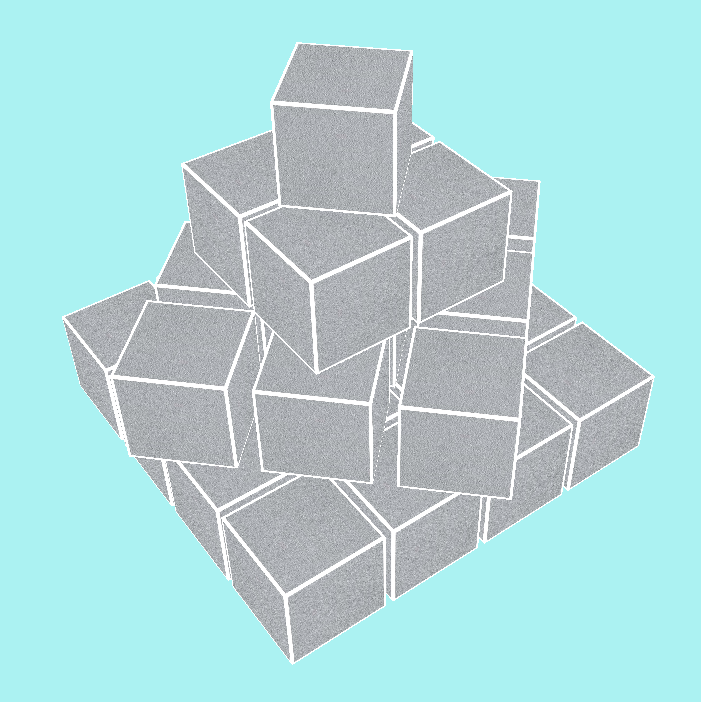
\includegraphics[width=.95\linewidth]{figures/qtp1-shape2-model.png}
		\caption{Shape ID 2}
		\label{fig:qtp1-shape2-model}
	\end{subfigure}%
	\begin{subfigure}{.29167\textwidth}
		\centering
		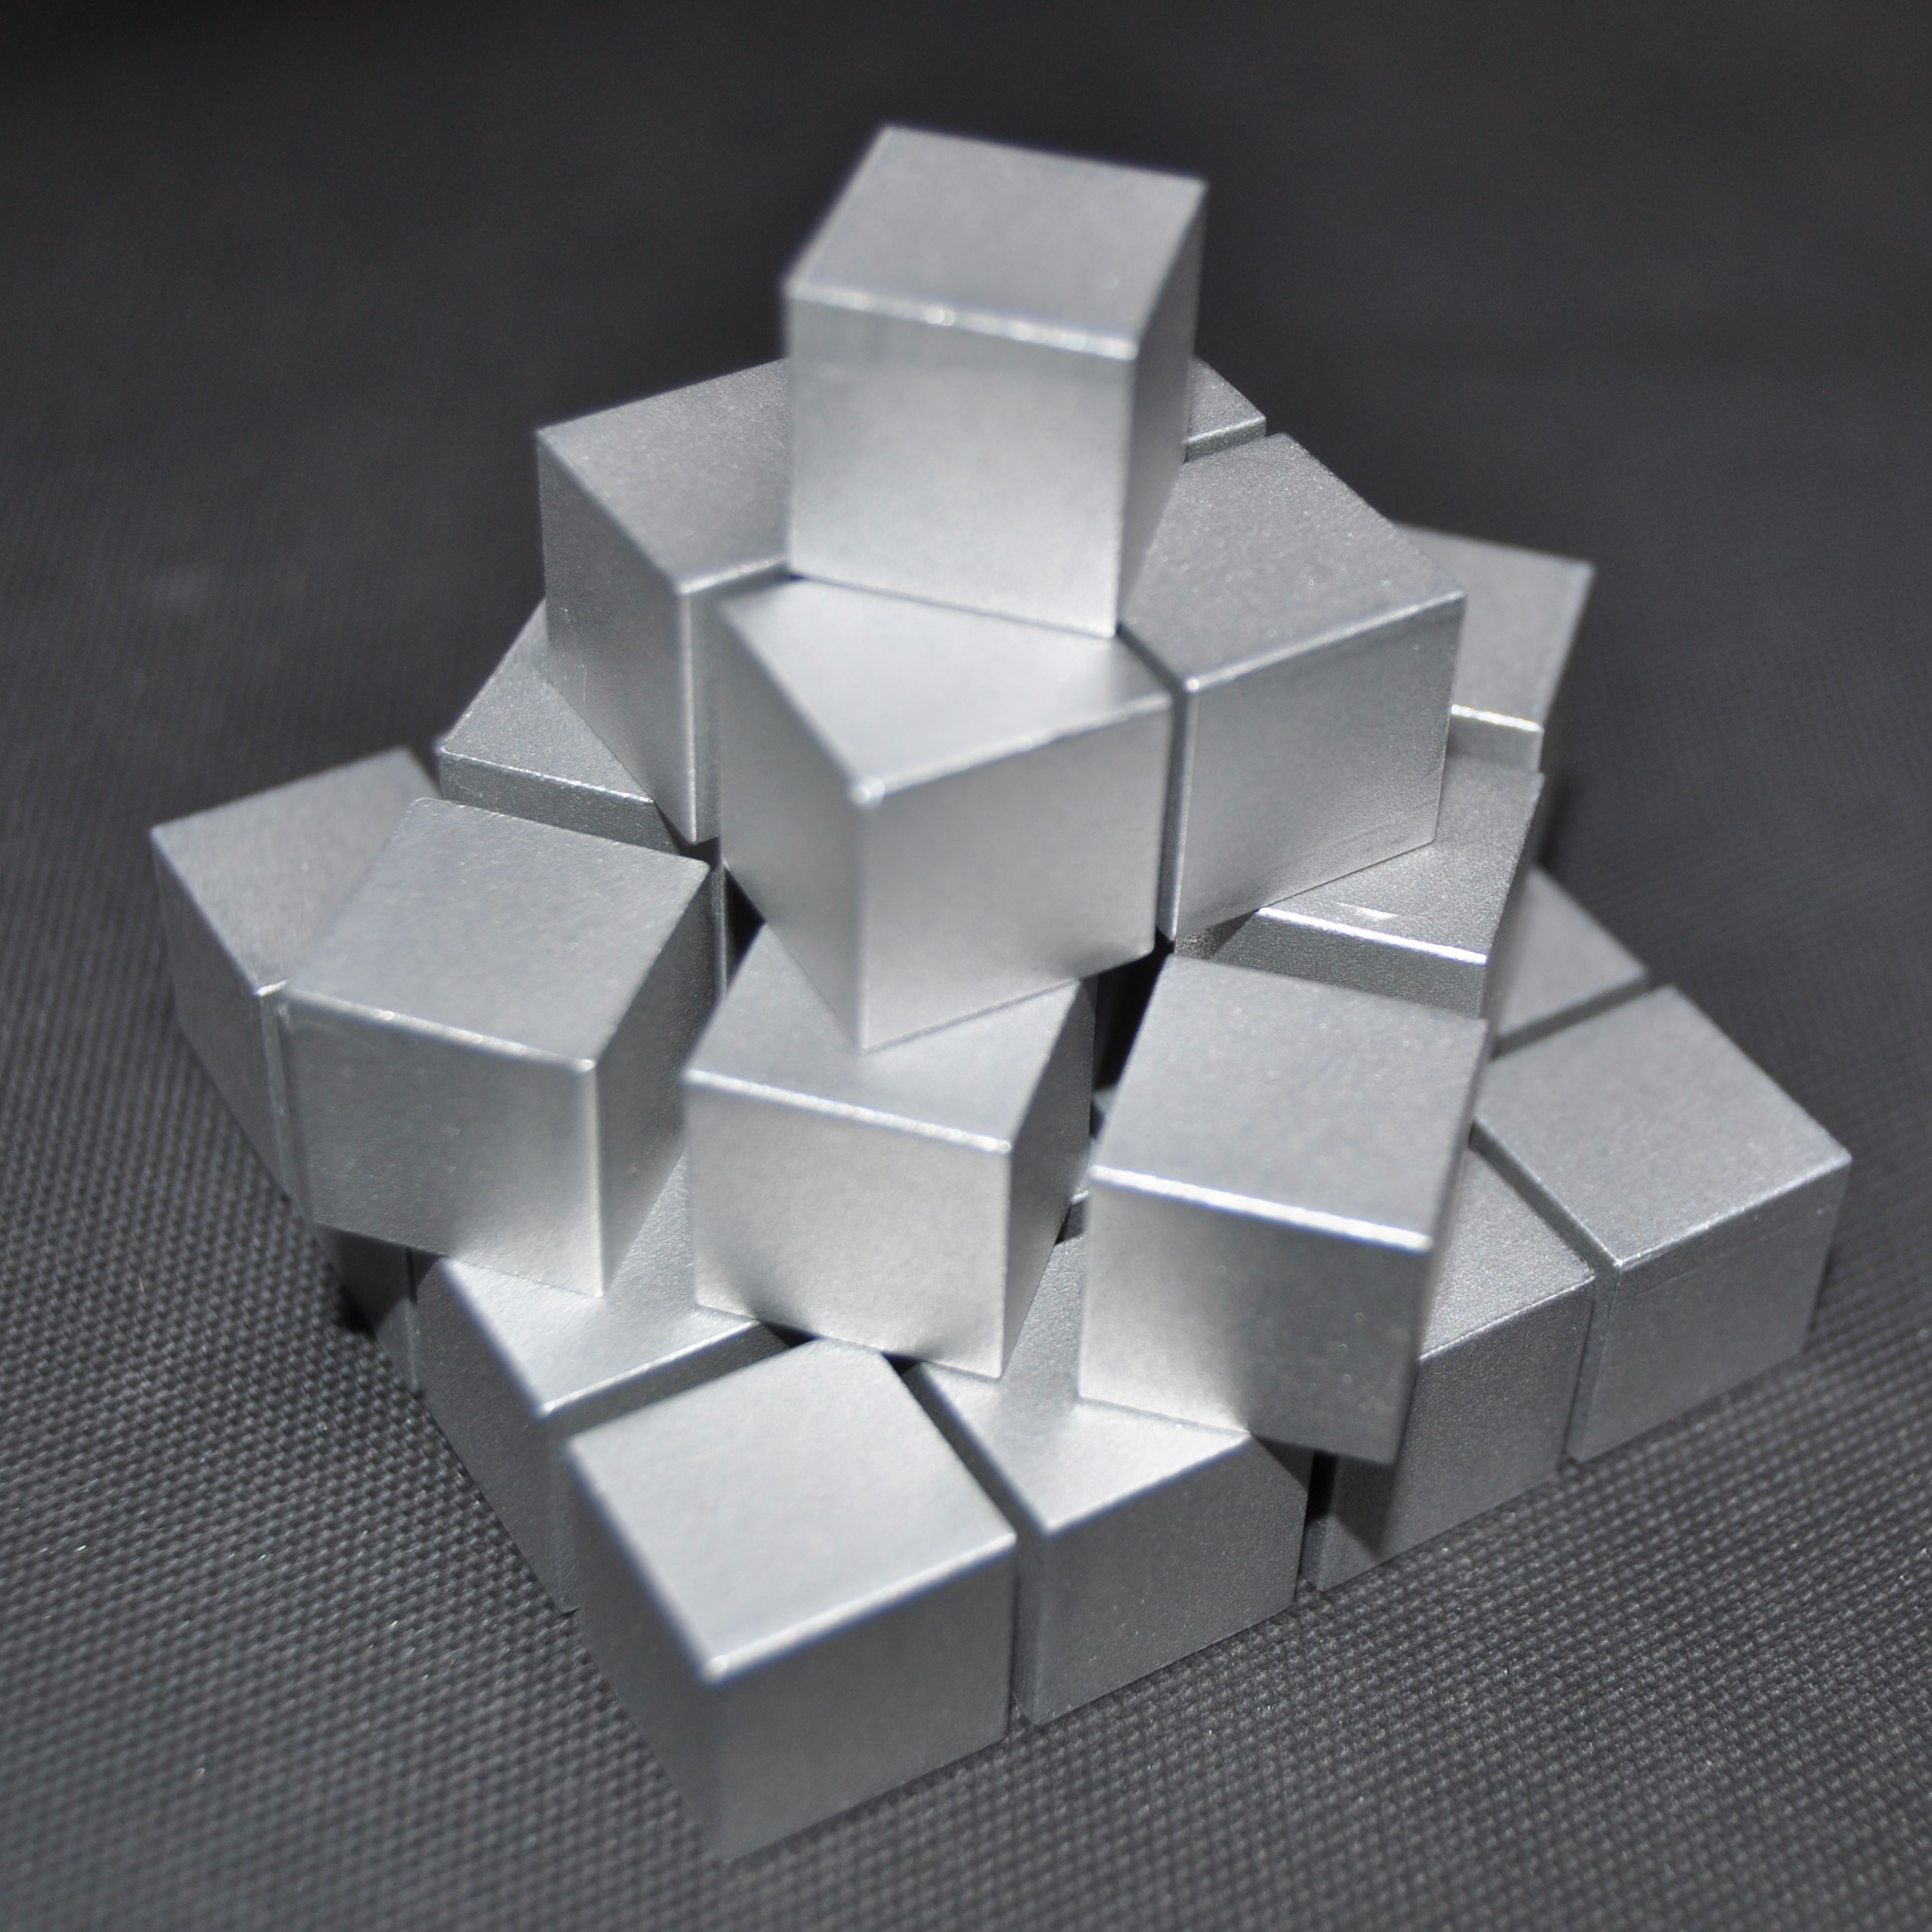
\includegraphics[width=.95\linewidth]{figures/qtp1-shape2.jpg}
		\caption{Shape ID 2}
		\label{fig:qtp1-shape2}
	\end{subfigure}% 
	\begin{subfigure}{.20833\textwidth}
		\centering
		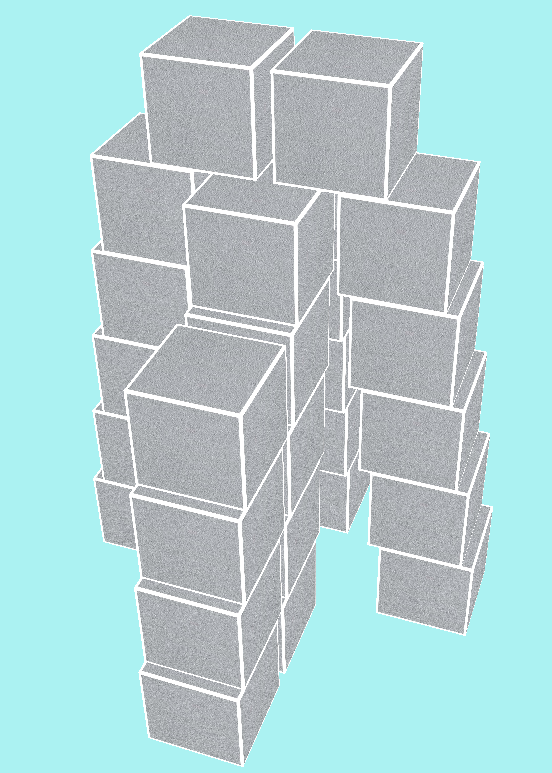
\includegraphics[width=.95\linewidth]{figures/qtp1-shape3-model.png}
		\caption{Shape ID 3}
		\label{fig:qtp1-shape3-model}
	\end{subfigure}%
	\begin{subfigure}{.20833\textwidth}
		\centering
		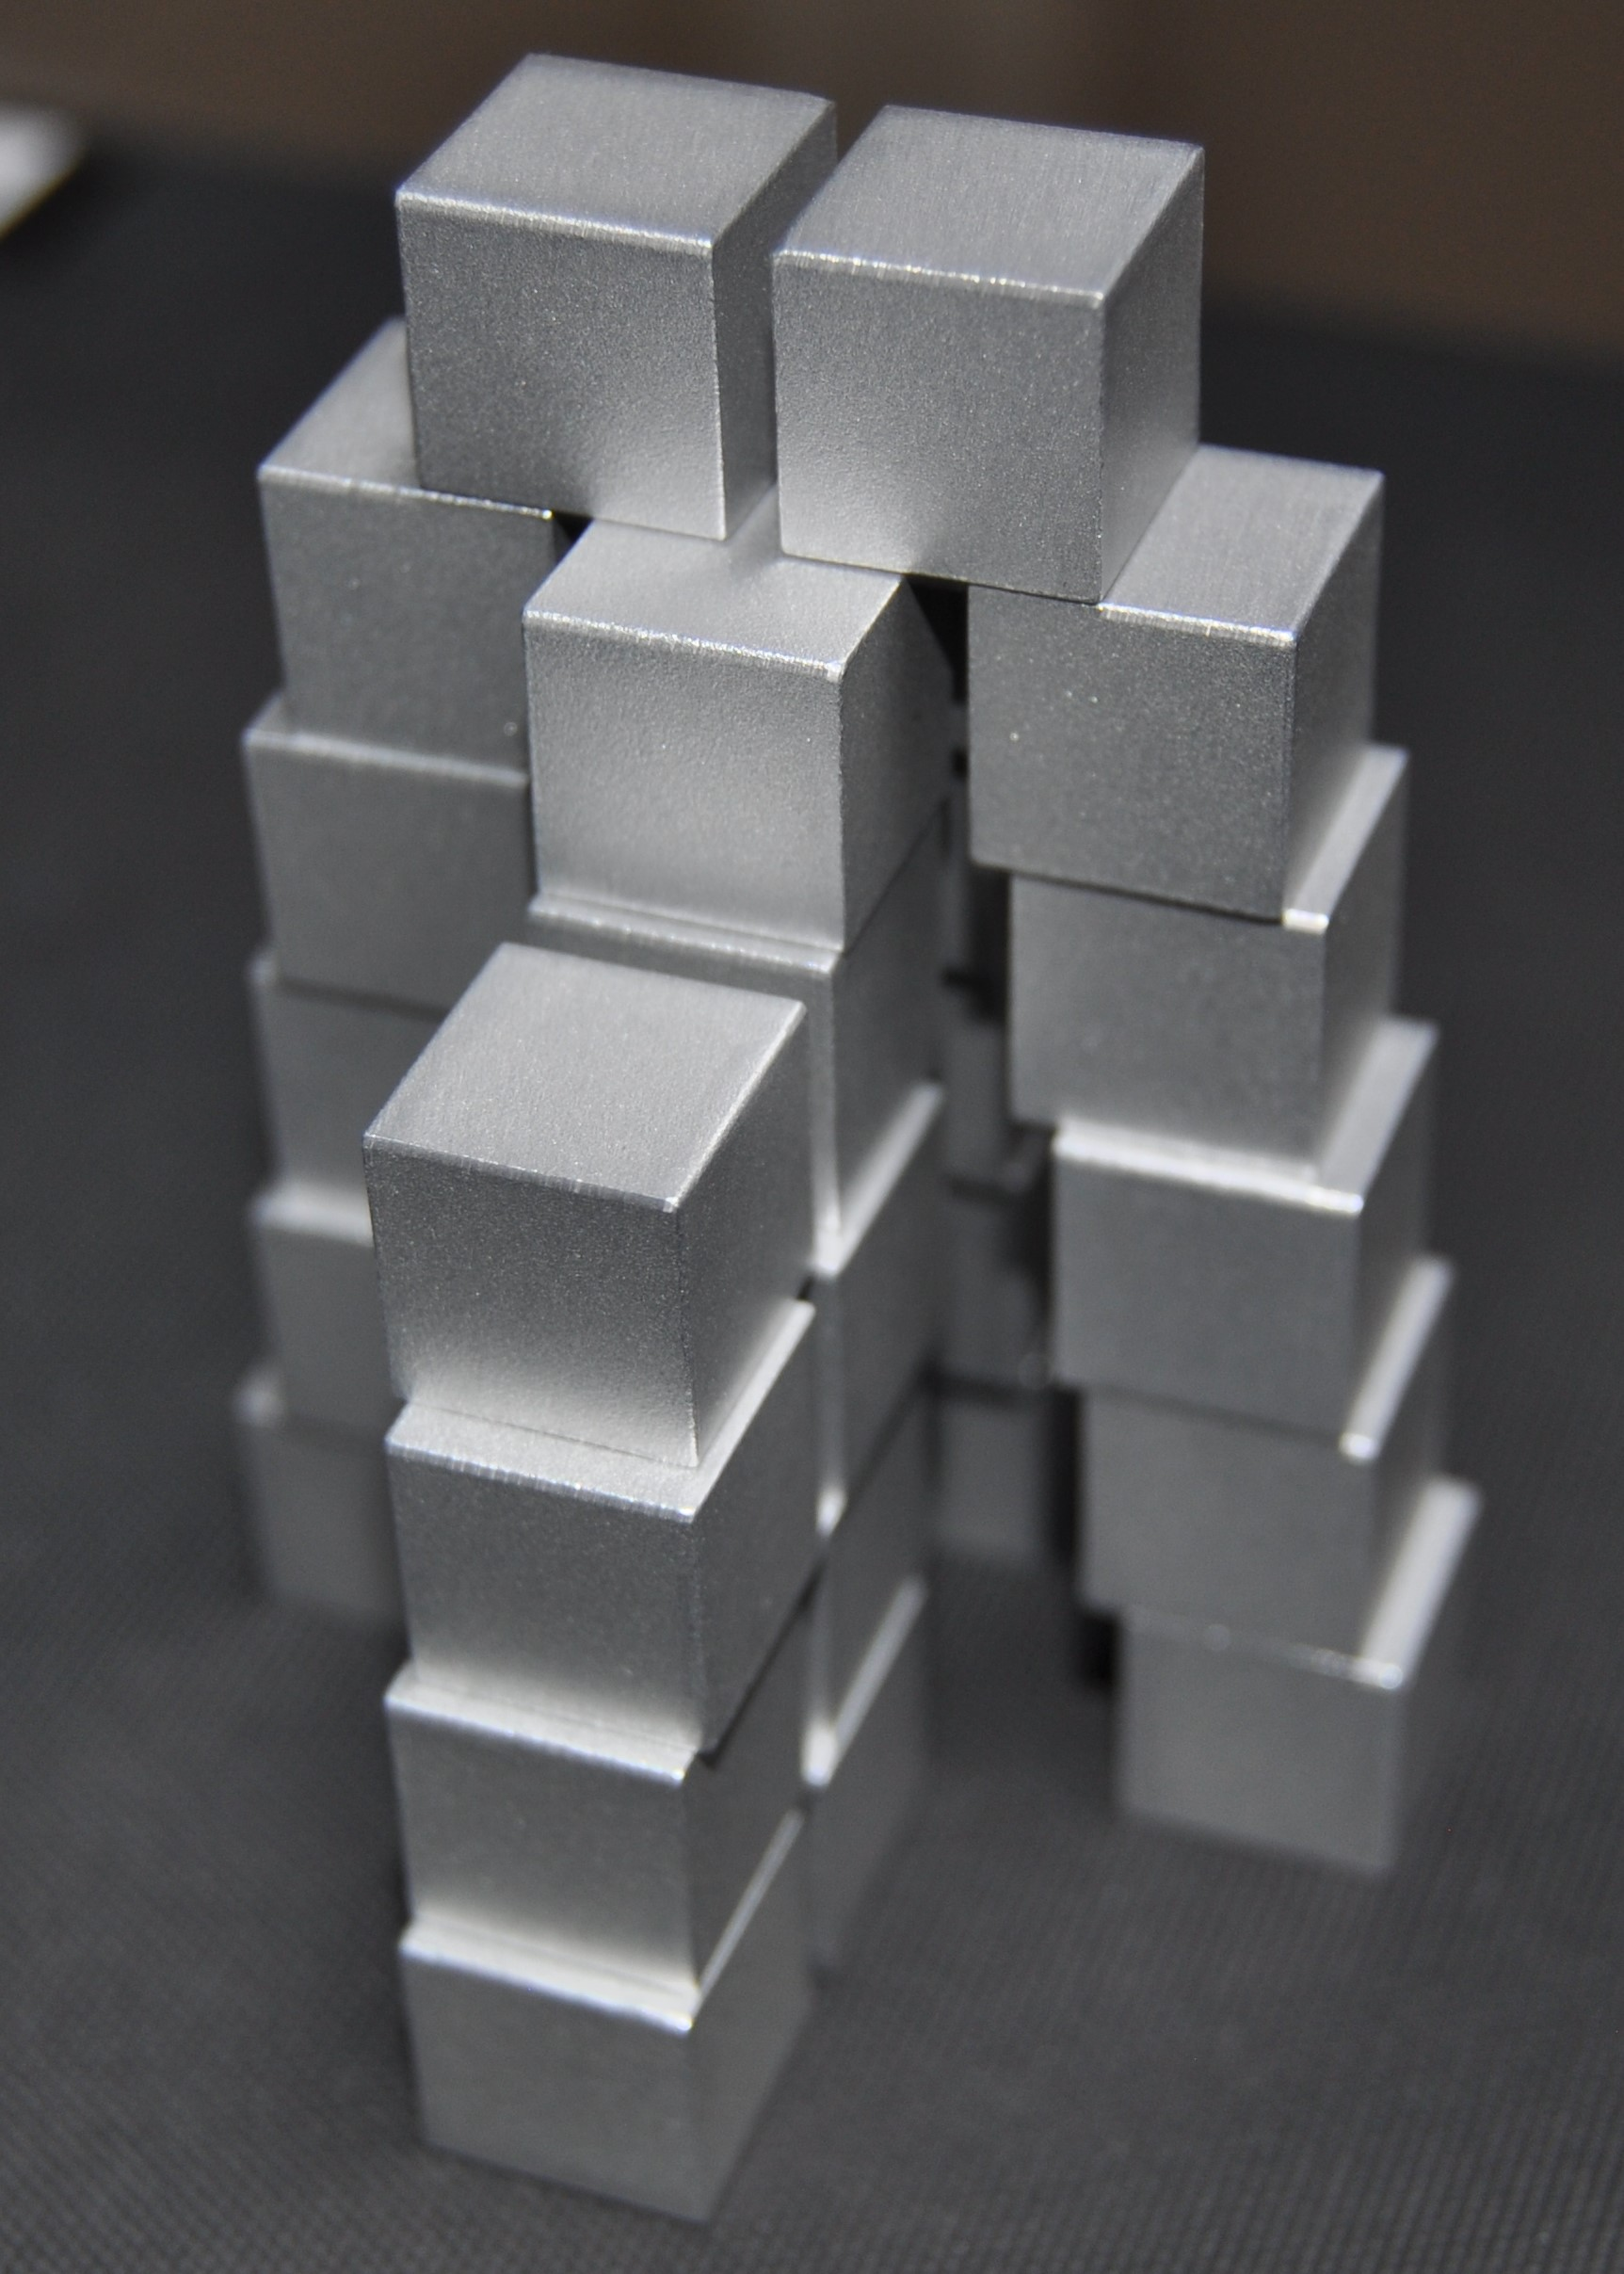
\includegraphics[width=.95\linewidth]{figures/qtp1-shape3.jpg}
		\caption{Shape ID 3}
		\label{fig:qtp1-shape3}
	\end{subfigure}
	\caption{3D shape models and corresponding shapes constructed by the system for qualification test 1.}
	\label{fig:qtp1-results}
\end{figure}

\textbf{Qualification Test 2: Test of system's capability to facilitate the definition of 3D shapes}

\textit{Objectives of the test or experiment}

The aim of this test is to determine if the system is capable of capturing and representing a user-specified 3D shape where the position of each constituent cube is specified along each Cartesian axis as well as the orientation about the z-axis.

\textit{Equipment used}

The following steps were carried out to execute this qualification test:

\begin{compactitem}
	\item PC,
	\item and \textit{PC System} software.
\end{compactitem}

\textit{Test setup and experimental parameters}

The following steps were completed in preparation for this qualification test:
\begin{compactitem}
	\item Start the system control software on the PC.
	\item Navigate to the \textit{Shape Design} view in the system control GUI.
\end{compactitem}

\textit{Steps followed in the test or experiment}

The following steps were carried out to execute this qualification test:

\begin{compactenum}
	\item Click on the \textit{Insert Cube} button in the \textit{Shape Design} view in the system control GUI.
	\item Verify a cube is displayed in the 3D shape display.
	\item Record the displayed x-axis position value for the cube.
	\item Translate the cube one step in the positive x-axis direction.
	\item Record the displayed x-axis position value for the cube.
	\item Translate the cube one step in the negative x-axis direction
	\item Record the displayed x-axis position value for the cube.
	\item Repeat steps 2 to 6 for translation along the y-axis.
	\item Repeat steps 2 to 6 for rotation about the z-axis.
	\item Click on the \textit{Insert Cube} button
	\item Verify an additional cube is added to the 3D shape display.
	\item Verify the cube can be translated along the x-, y-, and z-axis and rotated about the z-axis.
	\item Repeat steps 10 to 12 until 30 cubes are displayed in the 3D shape display.
\end{compactenum}

\textit{Results or measurements}

The cube linear step size on both the x- and y-axis in both the positive and negative directions was 0.1 mm. The cube rotational step size about the z-axis in both the positive and negative directions was 0.9$\degree$. 30 cubes were successfully displayed in the shape display. Each of the 30 cubes could be translated along each axis and rotated about the z-axis.

\textbf{Qualification Test 3: Test of end-effector's capability to manipulate cubes}

\textit{Objectives of the test or experiment}

The aim of this test is to determine if the end-effector is capable of maintaining a cube in its grip under motion when the robotic manipulator is at maximum acceleration. The test also aims to determine if the end-effector is able to maintain the cube in its grip for at least 20 seconds continuously and if it is able to grip and ungrip the cube.

\textit{Equipment used}

The following equipment was used to execute this qualification test:

\begin{compactitem}
	\item PC,
	\item \textit{PC System} software,
	\item \textit{Robotic Subsystem},
	\item USB Type A to micro USB connector cable,
	\item Digital stopwatch,
	\item and an aluminium cube with a side length of 12.6mm $\pm$0.05mm.
\end{compactitem}

\textit{Test setup and experimental parameters} 

The following steps were completed in preparation for this qualification test:

\begin{compactenum}
	\item Ensure the \textit{General System Initialisation} procedure has been completed.
	\item Navigate to the \textit{Construction} view in the system control GUI.
\end{compactenum}

\textit{Steps followed in the test or experiment}

The following steps were carried out to execute this qualification test:

\begin{compactenum}
	\item Place the cube in first position of the pre-defined \textit{source cube} locations.
	\item Click on the \textit{Execute QTP 3} button to initiate the robot's routine for this qualification test.
	\item Verify the robotic subsystem proceeds to grip the cube placed during the test setup.
	\item Start the stopwatch as the cube is lifted off the base plane by the robotic manipulator.
	\item Verify, the robot continuously between the extreme locations on each axis.
	\item Stop the stopwatch and record the elapsed time if the cube is dropped by the robot at any point during the robot's movement sequence up to 30 seconds.
	\item After 30 seconds halt the robot's movement sequence and record if the cube is still gripped by the robot.
	\item If the cube is still gripped by the robot, press the \textit{Release Actuator} button and record if the cube is released.
	\item Repeat steps 1 to 7 until a total of 10 iterations have been completed.
\end{compactenum}

\textit{Results or measurements}

The full results from this qualification test can be found in Table \ref{tab:techdoc-qtp3} in the technical documentation appendix. The following is a summary of these results:

\begin{compactitem}
	\item Iterations performed = 10,
	\item Number of iterations where cube was successfully gripped = 10,
	\item Number of iterations where the cube was dropped before 30 seconds = 0,
	\item Number of iterations where the move sequence was completed with the cube still gripped = 10,
	\item Number of iterations where the cube was successfully released on command = 10.
\end{compactitem}

\textit{Observations}

No unexpected events occurred during any of the movement iterations which were all completed successfully.

\textbf{Qualification Test 4: Measurement of robotic manipulator linear accuracy}

\textit{Objectives of the test or experiment}

The aim of this test is to determine the linear repeatability of the robotic manipulator's positioning along each Cartesian axis.

\textit{Equipment used}

The following equipment was used to execute this qualification test:

\begin{compactitem}
	\item PC,
	\item \textit{PC System} software,
	\item ImageJ image processing and analysis software,
	\item \textit{Robotic Subsystem},
	\item USB Type A to micro USB connector cable,
	\item Vertical flat-faced stand (see Figure \ref{fig:qtp4-z-axis-test-structure}),
	\item 2 sheets of plain white A4 paper,
	\item Digital caliper,
	\item 0.5mm Mechanical pencil,
	\item Electrical tape,
	\item and a Digital camera.
\end{compactitem}

\textit{Test setup and experimental parameters}

\begin{compactenum}
	\item Ensure the \textit{General System Initialisation} procedure has been completed.
	\item Navigate to the \textit{Construction} view in the system control GUI.
	\item Attach the mechanical pencil vertically and securely to the robot's \textit{End-Effector Assembly} using electrical tape as shown in Figure \ref{fig:qtp4-vertical-pencil}.
	\item Place the two sheets of plain white A4 paper on the base plane of the robot's workspace such that entire plane accessible by mechanical pencil tip is covered.
	\item Secure the paper sheets in place to the base plane using electrical tape.
\end{compactenum}

\begin{figure}[!ht]
	\centering
	\begin{subfigure}{.25\textwidth}
		\centering
		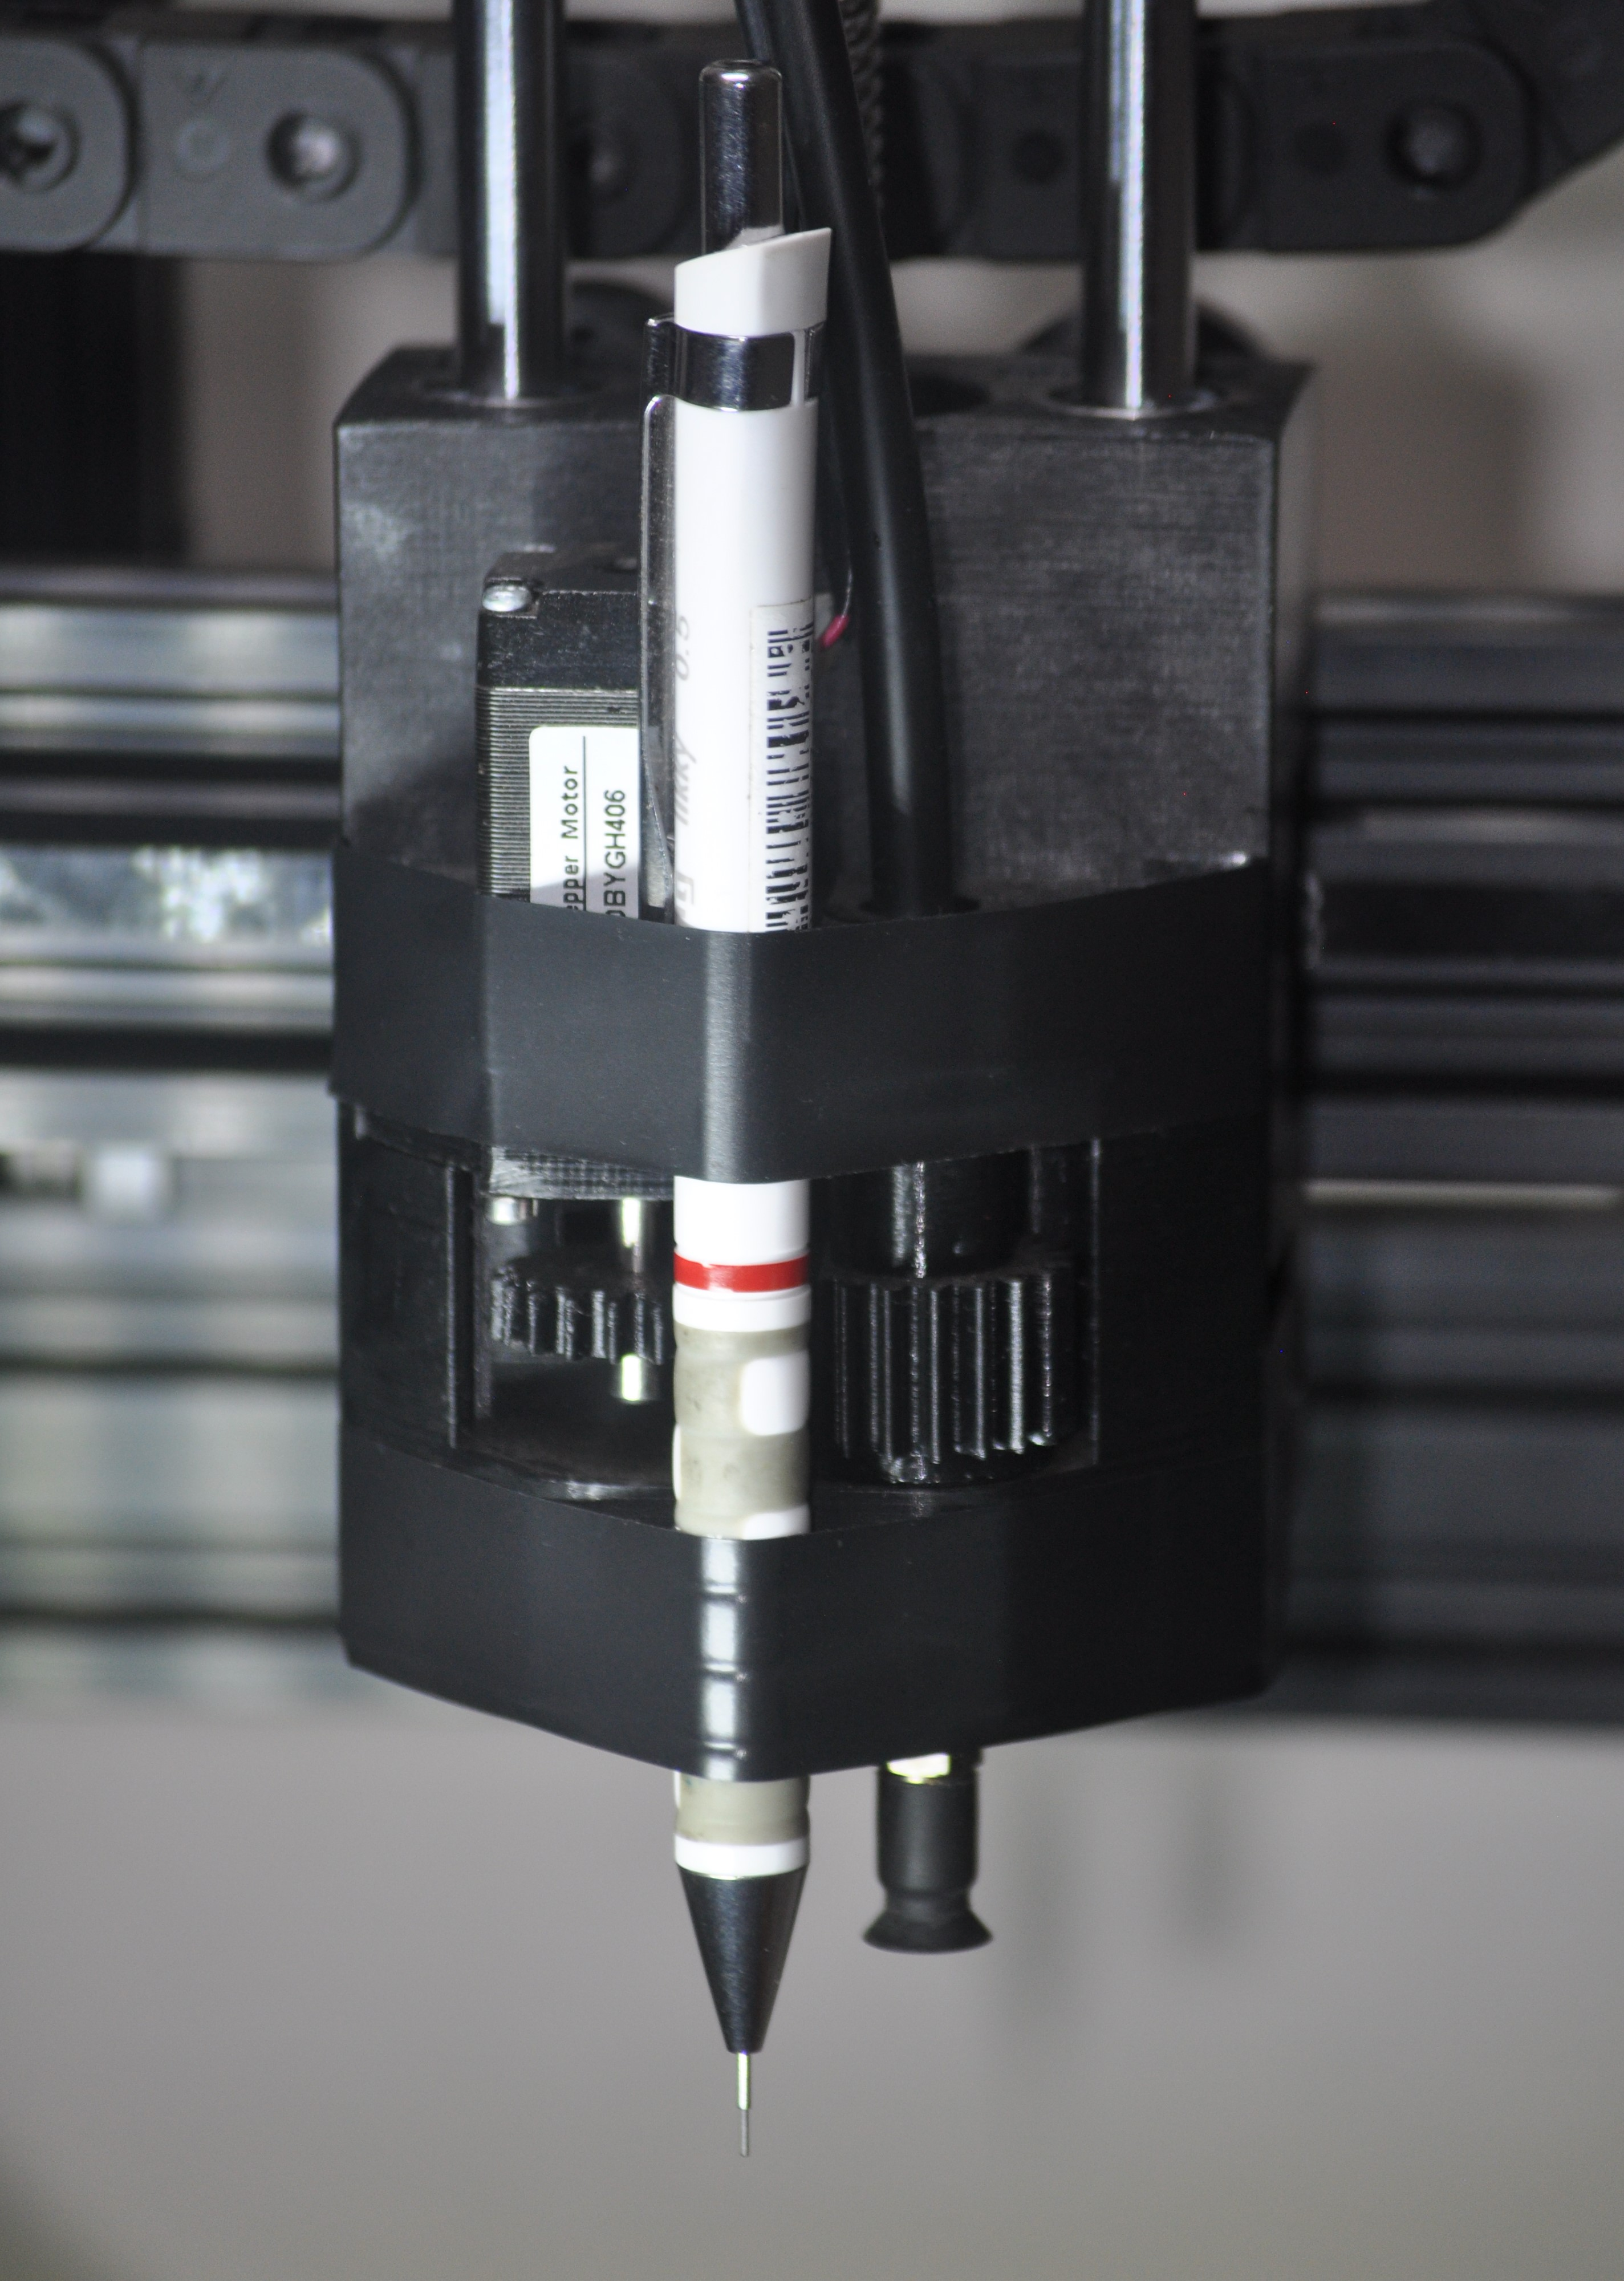
\includegraphics[width=0.95\linewidth]{figures/qualification-test-vertical-pencil.jpg}
		\caption{Vertical pencil}
		\label{fig:qtp4-vertical-pencil}
	\end{subfigure}%
	\begin{subfigure}{.53\textwidth}
		\centering
		\includegraphics[width=0.95\linewidth]{figures/qualification-test-horizontal-pencil.jpg}
		\caption{Horizontal pencil attachment}
		\label{fig:qtp4-horizontal-pencil}
	\end{subfigure}
	\begin{subfigure}{.21\textwidth}
		\centering
		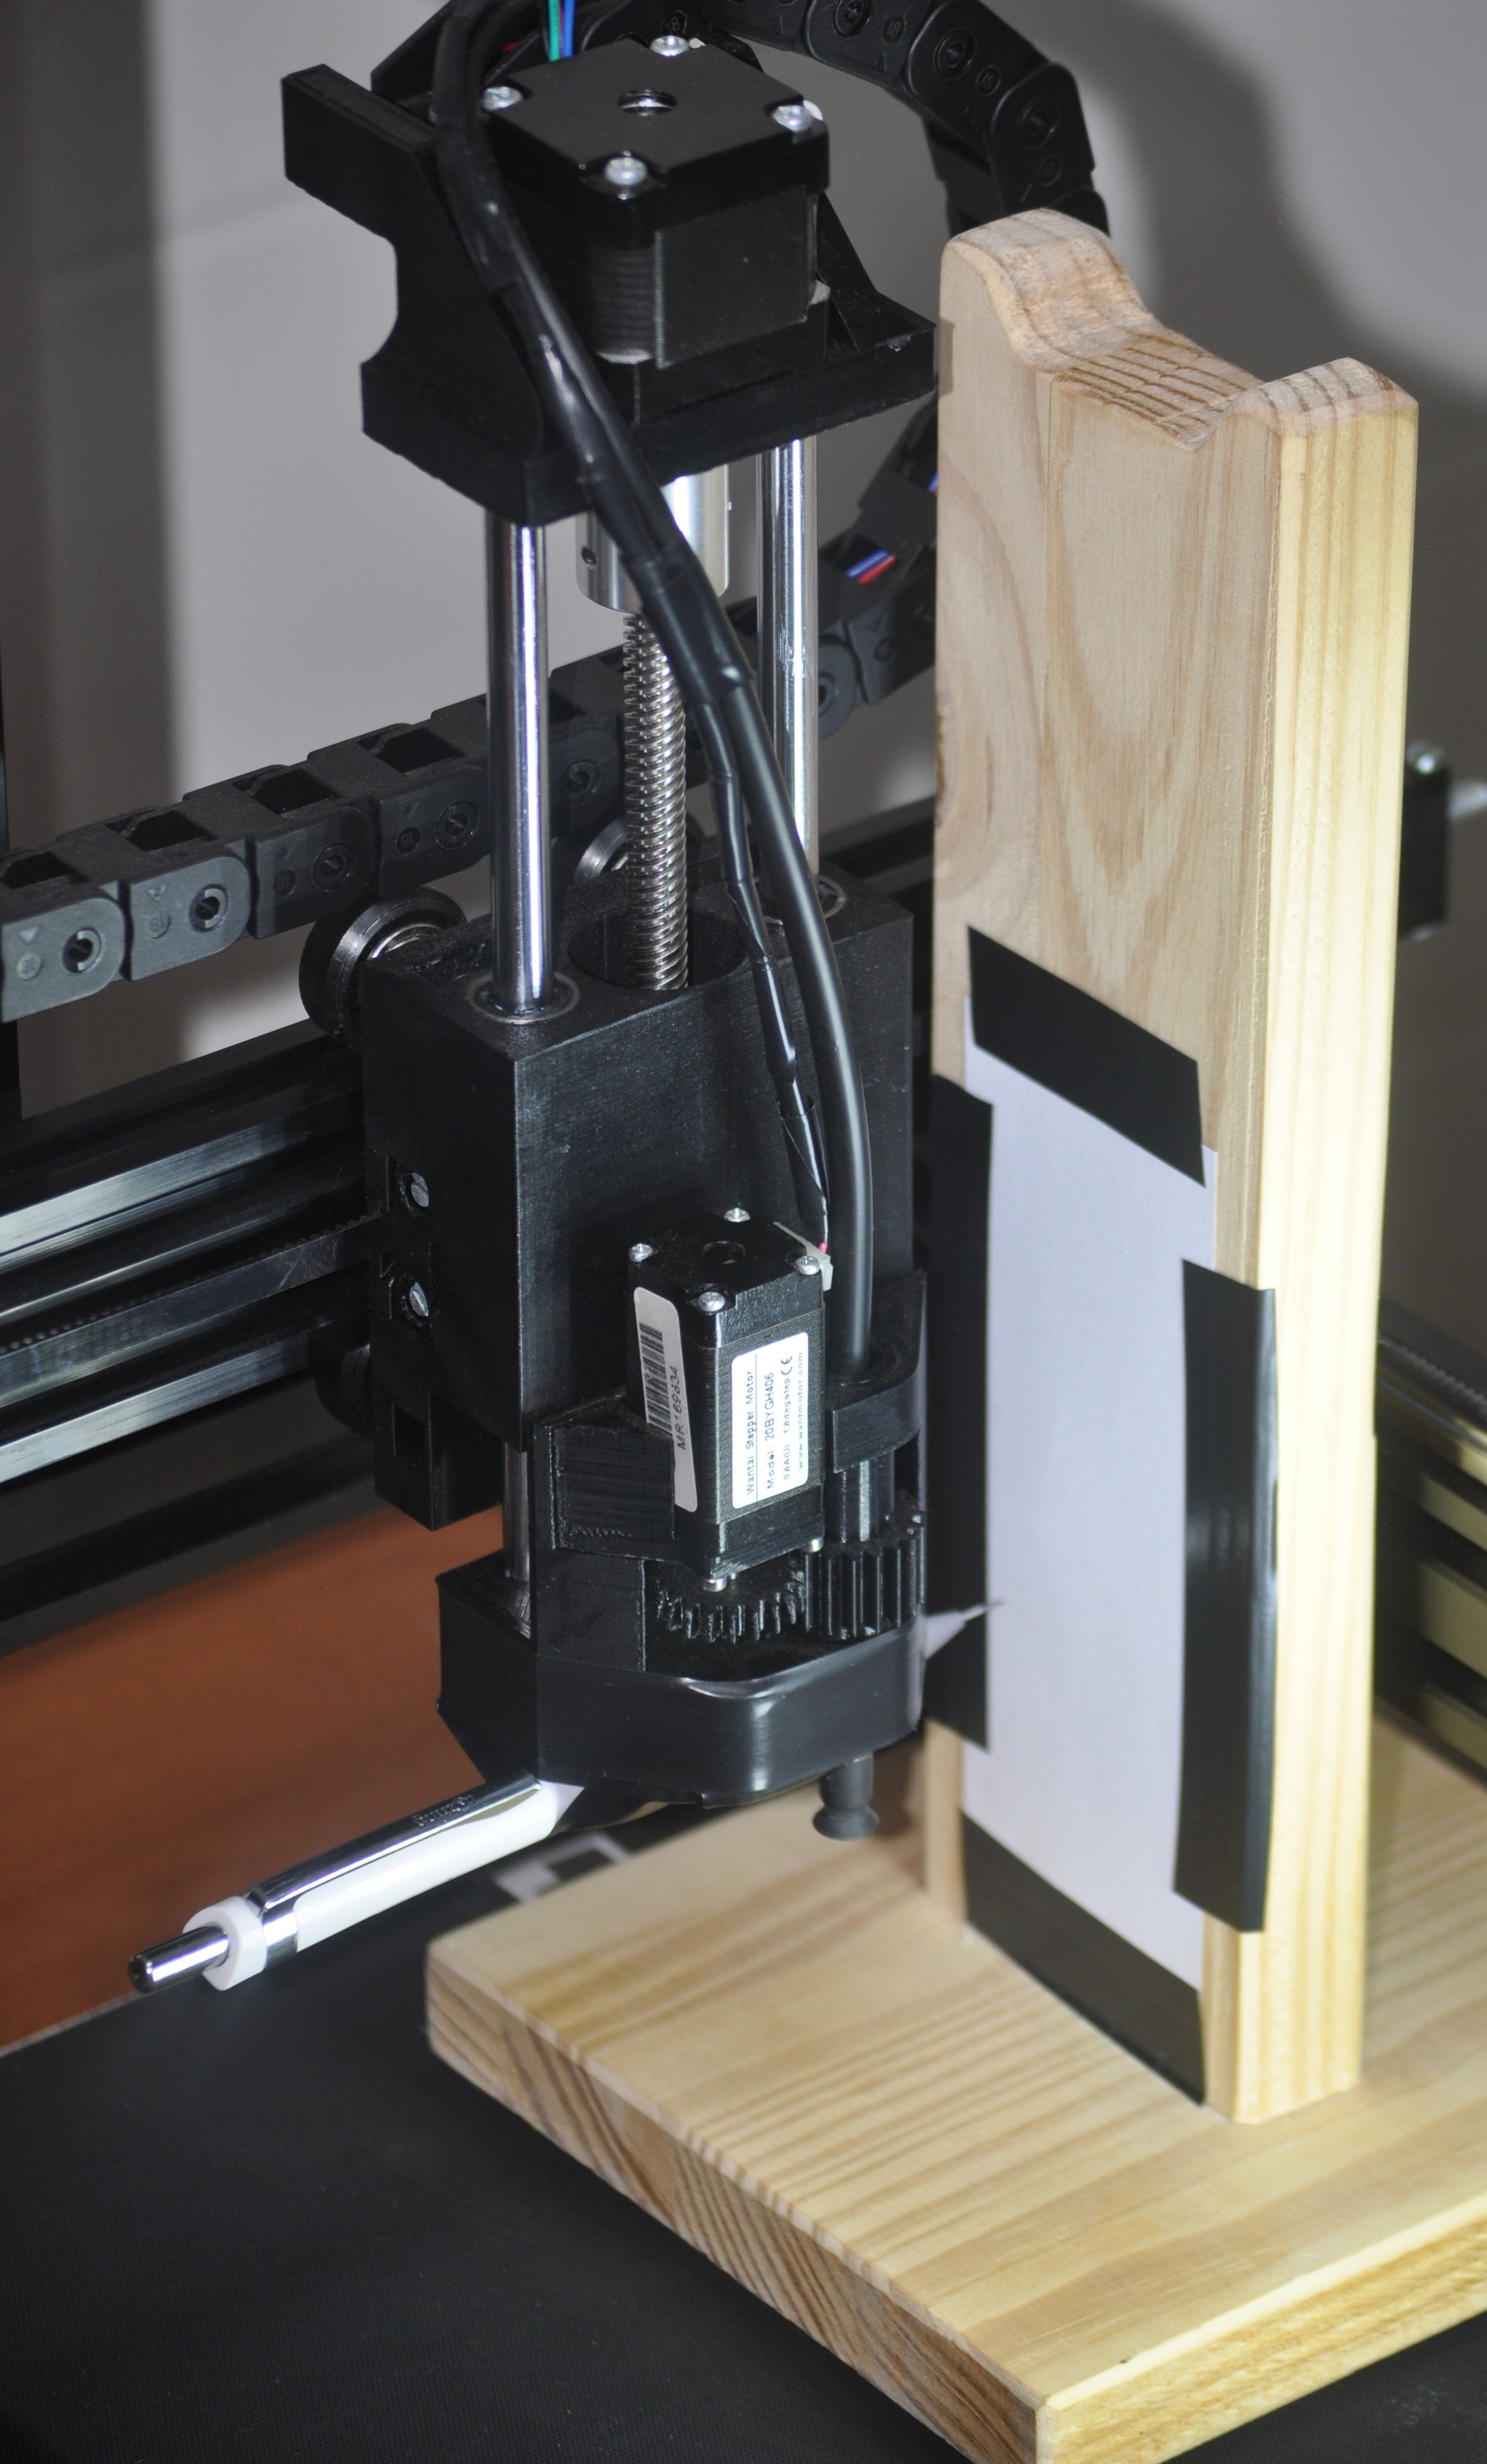
\includegraphics[width=0.95\linewidth]{figures/qualification-test-z-repeat-stand.jpg}
		\caption{Stand setup}
		\label{fig:qtp4-z-axis-test-structure}
	\end{subfigure}
	\caption{Experimental setup configuration used during qualification test 4.}
	\label{fig:qtp4-linear-repeatability-setup}
\end{figure}

\textit{Steps followed in the test or experiment}

The following steps were carried out to execute this qualification test:

\begin{compactenum}
	\item Using the position controls in the system GUI's \textit{Construction} view, iteratively reduce the z-position of the robot until the tip of the mechanical pencil touches the sheet of paper on the base plane firmly enough to leave a mark on the paper. Record this z-position in steps as $z_{mark}$.
	\item Let the x and y coordinates of the position where the robot's repeatability is being tested be denoted by $x_{test}$ and $y_{test}$ respectively. Let the x- and y- coordinates of the reference position to where the robot moves after making a mark be denoted by $x_{ref}$ and $y_{ref}$. Select these values as $x_{test}=0$, $y_{test}=0$, $x_{ref}=1015$ and $y_{ref}=1125$ steps.
	\item Move the robotic end-effector to position ($x_{test}$, $y_{test}$, $z_{mark}$ + 50) where the elements of this tuple refer to the x-, y- and z-position of the robot respectively.
	\item Decrease the z-position of the robotic end-effector to $z_{mark}$ to place a mark on the paper on the base plane.
	\item Increase the z-position of the robotic end-effector to $z_{mark}$ + 50 to remove the pencil tip from the paper.
	\item Move the robotic end-effector to the reference position ($x_{ref}$, $y_{ref}$, 2200) where the state tuple contains the target x-, y- and z-position of the robotic end-effector respectively.
	\item Repeat steps 3 to 6 until a total of 10 iterations have been completed for the given test position.
	\item Repeat steps 2 to 7 with  $x_{test}=1015$, $y_{test}=1125$, $x_{ref}=0$ and $y_{ref}=0$ steps.
	\item Repeat steps 2 to 7 with  $x_{test}=1015$, $y_{test}=0$, $x_{ref}=0$ and $y_{ref}=1125$ steps.
	\item Repeat steps 2 to 7 with  $x_{test}=0$, $y_{test}=0$, $x_{ref}=1015$ and $y_{ref}=0$ steps.
	\item Repeat steps 2 to 7 with  $x_{test}=507$, $y_{test}=562$, $x_{ref}=0$ and $y_{ref}=0$ steps to test the repeatability in the middle of the robot's workspace.
	\item Remove the and reattach the mechanical pencil horizontally and securely to the robot's \textit{End-Effector Assembly} using electrical tape as shown in Figure \ref{fig:qtp4-horizontal-pencil}.
	\item Attach a piece of plain white paper to the vertical surface of the flat-faced stand as shown in Figure \ref{fig:qtp4-z-axis-test-structure} and place the stand in the back right corner of the robot's workspace with the vertical face aligned with the zy plane.
	\item The z-repeatability for two z-planes are tested simultaneously by moving between the two planes and marking a point on the paper for each plane. Let the lower plane be denoted by $z_{lower}$ and the upper plane be denoted by $z_{upper}$. Select these values as $z_{lower}=500$ and $z_{upper}=2300$ steps.
	\item Position the robotic end-effector such that the tip of the mechanical pencil touches the sheet of paper on the vertical stand surface firmly enough to leave a mark on the paper. Record the x- and y-position in steps as $x_{mark}$ and $y_{mark}$ respectively.
	\item Move the robotic end effector to ($x_{mark}$ - \textit{offset}, $y_{mark}$, $z_{lower}$) where \textit{offset}=50 steps when the vertical stand is facing left and \textit{offset}=-50 steps when facing right.
	\item Set the x-position of the robotic end-effector to $x_{mark}$ to mark the point on the paper.
	\item Set the x-position of the robotic end-effector to $x_{mark}$ - \textit{offset} to remove the pencil tip from the paper.
	\item Set the z-position of the robotic end-effector to $z_{upper}$.
	\item Set the x-position of the robotic end-effector to $x_{mark}$ to mark the point on the paper.
	\item Set the x-position of the robotic end-effector to $x_{mark}$ - \textit{offset} to remove the pencil tip from the paper.
	\item Repeat steps 16 to 21 until 10 iterations have been performed.
	\item Repeat steps 15 to 22 with the vertical stand in the back left, front right, front left and centre of the robot's workspace.
	\item For each cluster of point markings on each sheet of paper, set the digital caliper to 2.00 mm and press the tips of the caliper into the sheet of paper near the point such that the paper is indented with the 2.00 mm reference mark.
	\item Take a photo of each cluster of point markings using the digital camera.
	\item Use the ImageJ image processing software to isolate the cluster of point markings.
	\item Using ImageJ, calibrate for length using the 2.00mm reference indents and measure the spread of the markings in the x, y and z directions depending on the sample. Record these measurements.
\end{compactenum}

\textit{Results or measurements}

The full results from this qualification test can be found in Tables \ref{tab:techdoc-qtp4-xy1}, \ref{tab:techdoc-qtp4-xy2} and \ref{tab:techdoc-qtp4-z1} in the technical documentation appendix. Tables \ref{tab:qtp4-xy} and \ref{tab:qtp4-z} show a reduced set of these results:

\begin{table}[H]
	\renewcommand{\arraystretch}{1.3}
	\centering
	\begin{tabular}{|>{\raggedright}m{1.5cm}|>{\raggedright}m{1.9cm}|>{\raggedright}m{1.9cm}|>{\raggedright}m{1.9cm}|>{\raggedright}m{2.5cm}|>{\raggedright\arraybackslash}m{2.5cm}|}
		\hline
		\textbf{Sample Set} & \textbf{X Position (steps)} & \textbf{Y Position (steps)} & \textbf{Z Position (steps)} & \textbf{X Points Range (mm)} & \textbf{Y Points Range (mm)} \\
		\hline
		1 & 0    & 0    & 0 & 0,2463 & 0,2028   \\
		\hline
		2 & 0    & 1125 & 0 & 0,4532 & 0,3610 \\
		\hline
		3 & 507  & 562  & 0 & 0,4530 & 0,3473 \\
		\hline
		4 & 1015 & 0    & 0 & 0,4211 & 0,3256 \\
		\hline
		5 & 1015 & 1125 & 0 & 0,3064 & 0,2323 \\
		\hline
	\end{tabular}
	\caption{\label{tab:qtp4-xy}Range of points along the x- and y-axis measured from the point cluster images for qualification test 4.}
\end{table}

\begin{table}[H]
	\renewcommand{\arraystretch}{1.3}
	\centering
	\begin{tabular}{|>{\raggedright}m{1.5cm}|>{\raggedright}m{1.9cm}|>{\raggedright}m{1.9cm}|>{\raggedright}m{1.9cm}|>{\raggedright}m{1.8cm}|>{\raggedright}m{1.6cm}|>{\raggedright\arraybackslash}m{1.6cm}|}
		\hline
		\textbf{Sample Set} & \textbf{X Position (steps)} & \textbf{Y Position (steps)} & \textbf{Z Position (steps)} & \textbf{Reference Length (pixels)} & \textbf{Z Points Range (pixels)} & \textbf{Z Points Range (mm)} \\
		\hline
		1 & 852 & 70  & 500  & 60,001 & 23     & 0,7666 \\ \hline
		2 & 852 & 70  & 2300 & 61,26  & 19,96  & 0,6516 \\ \hline
		3 & 502 & 400 & 500  & 60,962 & 18,506 & 0,6071 \\ \hline
		4 & 502 & 400 & 2300 & 60,705 & 15,173 & 0,4998 \\ \hline
		5 & 194 & 700 & 500  & 60,397 & 17,557 & 0,5813 \\ \hline
		6 & 194 & 700 & 2300 & 60,27  & 19     & 0,6304 \\ \hline
	\end{tabular}
	\caption{\label{tab:qtp4-z}Range of points along the z-axis measured from the point cluster images for qualification test 4.}
\end{table}

\textit{Observations}

The main observation that was made during the executing of this qualification test was that the size of the pencil lead used to mark the points was similar to the range of the points distribution along all axes. No deviation among the 10 points per sample was observable with the naked eye.

\textit{Statistical analysis}

The mean and maximum range of the points along each axis were computed across the sample sets and are shown in Table \ref{tab:qtp4-stats}.

\begin{table}[H]
	\renewcommand{\arraystretch}{1.3}
	\centering
	\begin{tabular}{|>{\raggedright}m{3cm}|>{\raggedright}m{2cm}|>{\raggedright}m{2cm}|>{\raggedright\arraybackslash}m{2cm}|}
		\hline
		\textbf{Statistic} & \textbf{X Axis} & \textbf{Y Axis} & \textbf{Z Axis} \\ \hline
		\textit{Mean (mm)} & 0.3760 & 0.2938  & 0.6229 \\ \hline
		\textit{Maximum (mm)} & 0.4532 & 0.3610  & 0.7666 \\ \hline
	\end{tabular}
	\caption{\label{tab:qtp4-stats} Mean and maximum range for each axis across all the sample sets.}
\end{table}

\textbf{Qualification Test 5: Measurement of robotic manipulator's rotational accuracy}

\textit{Objectives of the test or experiment}

The aim of this test is to determine the rotational repeatability of the robotic manipulator rotational positioning about the z-axis.

\textit{Equipment used}

The following equipment was used to execute this qualification test:

\begin{compactitem}
	\item PC,
	\item \textit{PC System} software
	\item \textit{Robotic Subsystem},
	\item USB Type A to micro USB connector cable,
	\item an aluminium cube with a side length of 12.6mm $\pm$0.05mm,
	\item 25 x 20 grid of 10mm squares printed on a sheet of white A4 paper,
	\item Digital caliper,
	\item Electrical tape,
	\item and a 30 cm ruler.
\end{compactitem}

\textit{Test setup and experimental parameters}

The following steps were completed in preparation for this qualification test:

\begin{compactenum}
	\item Ensure the \textit{General System Initialisation} procedure has been completed.
	\item Navigate to the \textit{Construction} view in the system control GUI.
	\item Place the grid paper approximately in the centre of the robot's workspace. The grid does not need to be aligned with the robot's coordinate system.
	\item Secure the grid paper in place to the base plane using electrical tape as shown in Figure \ref{fig:qtp5-orientation-grid}.
\end{compactenum}

\begin{figure}[!ht]
	\centering
	\includegraphics[width=0.7\linewidth]{figures/robot-white-grid.jpg}
	\caption{Placement of grid in the robot's workspace to facilitate the measurement of the z-axis rotational repeatability.}
	\label{fig:qtp5-orientation-grid}
\end{figure}

\textit{Steps followed in the test or experiment}

The following steps were carried out to execute this qualification test:

\begin{compactenum}
	\item Choose any one of the 250 mm long grid lines and align the ruler with the line. Press down on the ruler so that the ruler does not shift from this position.
	\item Place the cube on the base plane and use the ruler to align the cube with the 250mm long grid line.
	\item Remove the ruler without disturbing the position or the orientation of the cube.
	\item Use the robot position controls in the \textit{Construction} view of the system control GUI to align the end-effector suction cup with the top of the cube.
	\item Set the rotational step position of the end-effector to 0 steps.
	\item Use the robot position and actuation controls in the \textit{Construction} view of the system control GUI to pick up the cube slightly above the base plane.
	\item Set the robotic end-effector's rotational step position to either 78 steps (odd iterations) or -78 steps (even iterations).
	\item Set the robotic end-effector's rotational step position back to 0 steps.
	\item Use the robot controls to move the cube vertically downwards, place the cube on the base plane and release the cube.
	\item Move the robotic end-effector vertically upwards and to a position that does not restrict access to the robot's workspace.
	\item Press down on the top face of the cube to preserve its orientation and position. 
	\item Use the face nearest to the 250 mm grid line to align the ruler against the cube. Press down on the ruler to preserve the ruler's orientation and position.
	\item Remove the cube from the robot's workspace.
	\item Let the first and last 200 mm long grid lines be denoted by $y_0$ and $y_1$ respectively. Use the placed ruler to draw a line that extends the full length of the grid and intersects with $y_0$ and $y_1$.
	\item Repeat steps to 1 to 14 until a total of 18 iterations have been completed using a different 250 mm grid line in each instance.
	\item Using the digital caliper, measure the deviation of the intersection of for each drawn line with $y_0$ from the intersection of the corresponding 250 mm grid line with $y_0$. Repeat this with $y_1$.
	\item Calculate $\phi$, the angle of each drawn line with respect to the corresponding 250 mm grid line as
	
\begin{equation}
	\phi=\arctan\frac{\delta_0-\delta_1}{\Delta x},
\end{equation}

	where $\delta_0$ and $\delta_1$ are the intersection deviations on $y_0$ and $y_1$ respectively while $\Delta x$ is the length of the 250 mm grid line
	\item Record these results.
\end{compactenum}

\textit{Results or measurements}

The full results from this qualification test can be found in Table \ref{tab:techdoc-qtp5-z-rot1} in the technical documentation appendix. The following is a summary of these results:

\textit{Observations}

Notable position offsets of the axis of rotation were observed during the rotation of the cube as a result from the end-effector gear surface being uneven.

\textit{Statistical analysis}

The mean angular deviation magnitude, maximum deviation and deviation bias was computed for all 18 angular deviation samples. These results are as follows:

\begin{compactitem}
	\item Mean angular deviation = 0.3153$\degree$,
	\item Maximum angular deviation = 0.8132$\degree$,
	\item Angular deviation bias = 0.08404$\degree$.
\end{compactitem}

\textbf{Qualification Test 6: Measurement of computer vision cube detection accuracy}

\textit{Objectives of the test or experiment}

The aim of this test is to determine the accuracy of the computer vision system in detecting and localising cubes whose faces are visible from a vertical perspective. Specifically, the test aims to determine the accuracy of the linear localisation along the x-axis and y-axis as well as the rotational pose estimation about the z-axis.

\textit{Equipment used}

The following equipment was used to execute this qualification test:

\begin{compactitem}
	\item PC,
	\item \textit{PC System} software
	\item \textit{Robotic Subsystem},
	\item USB Type A to micro USB connector cable,
	\item Logitech C920 HD Pro Webcam,
	\item 19 Aluminium cubes with side lengths of 12.6mm $\pm$0.05mm,
	\item Mechanical pencil,
	\item Matte black paper,
	\item Electrical tape,
	\item and a 30 cm ruler.
\end{compactitem}

\textit{Test setup and experimental parameters}

The following steps were completed in preparation for this qualification test:

\begin{compactenum}
	\item Place the matte black paper on the base plane of the robot's workspace and secure it in place using the electrical tape.
	\item Navigate to the \textit{Construction} view in the system control GUI.
	\item Move the robotic end-effector to the four extreme points on the base plane of the workspace and mark these point on the black paper using the mechanical pencil.
	\item Draw four lines to join these points to form a rectangle on the black paper using the mechanical pencil and ruler. Using the ruler, mark every 10 mm on each of the four lines.
\end{compactenum}

\textit{Steps followed in the test or experiment}

The following steps were carried out to execute this qualification test:

\begin{compactenum}
	\item Using the 10 mm markings as reference, place the ruler across the robot's workspace at an angle of 0$\degree$ with the x-axis of the robot's coordinate system. Do this at a number of positions. In each instance, press the ruler down firmly to preserve it's orientation and position.
	\item For each ruler placement, place a number of cubes by using the ruler to ensure the angle of each cube with with respect to the x-axis is 0$\degree$. Continue this process until 16 cubes have been placed.
	\item Using the robot position control in the system control GUI, align the suction cup of the robotic end-effector with the centre of the top face of each cube. Record the robotic end-effector's x and y coordinates when aligned with each cube. These are taken as the known world coordinate's of each cube.
	\item Click the \textit{Process Scene} button in the \textit{Construction} view of the GUI to trigger a capture and process action from the \textit{Vision System}.
	\item Record the position and orientation of each cube as estimated by the \textit{Vision System}.
	\item Repeat steps 1 to 5 using a ruler angle of 45 $\degree$ and a total of 19 cubes.
\end{compactenum}

\textit{Results or measurements}

The full results from this qualification test can be found in Tables \ref{tab:techdoc-qtp6-set1} and \ref{tab:techdoc-qtp6-set2} in the technical documentation appendix.

\textit{Observations}

A degree of misalignment was observed between the position of the cube as estimated by the computer vision component and the actual position of the cube based on the position of the end-effector. Furthermore, a degree of high-frequency noise was observed in the computer vision's estimate of the corner positions of cubes.

\textit{Statistical analysis}

The mean error magnitude, error bias and maximum error for the linear x-axis, linear y-axis and rotational z-axis were computed across all the cube samples and are shown in Table \ref{tab:qtp6-stats}. Furthermore, the linear error for the x- and y- axis as is shown in Figures \ref{fig:qtp6-x-axis-error} and \ref{fig:qtp6-y-axis-error} using colour on a per cube point basis with the points plotted as a scatter plot of the robot's workspace.

\begin{table}[H]
	\renewcommand{\arraystretch}{1.3}
	\centering
	\begin{tabular}{|>{\raggedright}m{3cm}|>{\raggedright}m{2.5cm}|>{\raggedright}m{2.5cm}|>{\raggedright\arraybackslash}m{3.5cm}|}
		\hline
		\textbf{Statistic} & \textbf{X Axis (mm)} & \textbf{Y Axis (mm)} & \textbf{Z Axis Rotation ($\degree$)} \\ \hline
		\textit{Mean Error Magnitude} & 0.4914 & 0.4971  & 0.9114 \\ \hline
		\textit{Error Bias} & -0.32 & 0.1314  & 0.3783 \\ \hline
		\textit{Maximum Error} & 1.4 & 1.2  & 3.5 \\ \hline
	\end{tabular}
	\caption{\label{tab:qtp6-stats} \textit{Vision System} cube detection mean error magnitude, error bias and maximum error for the linear x-axis, linear y-axis and rotational z-axis.}
\end{table}

\begin{figure}[!ht]
	\centering
	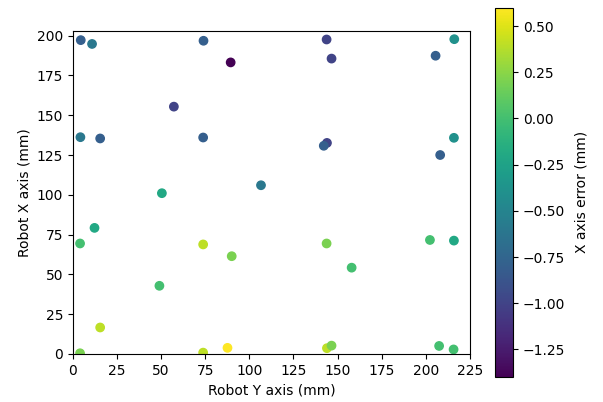
\includegraphics[width=0.7\linewidth]{figures/qtp6-x-axis-error.png}
	\caption{\textit{Vision System} cube position detection error along the x-axis.}
	\label{fig:qtp6-x-axis-error}
\end{figure}
\begin{figure}[!ht]
	\centering
	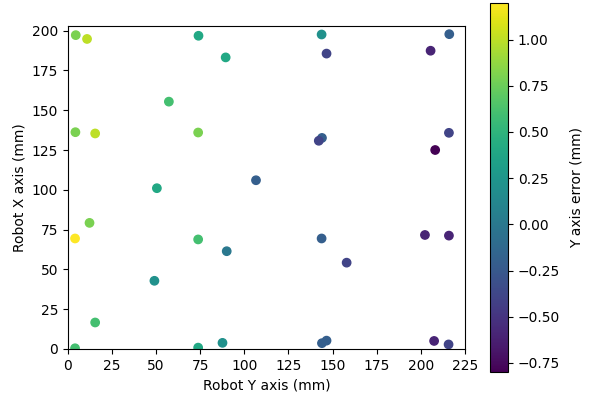
\includegraphics[width=0.7\linewidth]{figures/qtp6-y-axis-error.png}
	\caption{\textit{Vision System} cube position detection error along the y-axis.}
	\label{fig:qtp6-y-axis-error}
\end{figure}

\textbf{Qualification Test 7: Test of system's capability to detect a dropped cube and and shape construction failure}

\textit{Objectives of the test or experiment}

The aim of this test is to determine if the system is capable of detecting when a cube has been dropped by the end-effector.

\textit{Equipment used}

The following equipment was used to execute this qualification test:

\begin{compactitem}
	\item PC,
	\item \textit{PC System} software
	\item \textit{Robotic Subsystem},
	\item USB Type A to micro USB connector cable,
	\item Logitech C920 HD Pro Webcam,
	\item and 30 Aluminium cubes with side lengths of 12.6mm $\pm$0.05mm.
\end{compactitem}

\textit{Test setup and experimental parameters}

The following steps were completed in preparation for this qualification test:

\begin{compactenum}
	\item Ensure the \textit{General System Initialisation} procedure has been completed.
	\item Navigate to the \textit{Construction} view in the system control GUI.
\end{compactenum}

\textit{Steps followed in the test or experiment}

The following steps were carried out to execute this qualification test:

\begin{compactenum}
	\item Click on the \textit{Load model} button and select the \textit{.cubeworld} an arbitrary 30 cube test shape file.
	\item Clear the \textit{Robotic Subsystem's} workspace and place the 30 cubes at the pre-defined \textit{source cube} locations.
	\item Click on the \textit{Start Construction} button in the system control software to initiate the construction process.
	\item For each of the first 5 cubes, click the \textit{Release Actuator} button in the system control software to force the robot to drop the cube while carrying the cube to the structure. Note whether the robot detects the dropped cube condition before in the GUI info log before proceeding with construction.
	\item For cubes 6 to 10, manually remove the cube from the grip of the end-effector during the robot's final downward movement to place the cube and place the cube in the robot's workspace.
	\item Note whether the robot detects the dropped cube condition before in the GUI info log before proceeding with construction.
	\item Repeat steps 5 to 6 with cubes 11 to 15, but remove the cube during the robot's horizontal motion while moving the cube to the structure.
	\item Repeat steps 5 to 6 with cubes 16 to 20, but remove the cube during the robot's upward motion after gripping the cube.
	\item Repeat steps 5 to 6 with cubes 21 to 25, but remove the cube while the robot is moving to grip the cube.
	\item After the 25th cube has been placed, push the structure under construction until at least 1 cube falls from the structure.
	\item Note whether the system detects a construction failure condition using the GUI info log.
	\item Repeat steps 1 to 11 with a different test shape structure until 5 iterations have been completed.
\end{compactenum}

\textit{Results or measurements}

The full results from this qualification test can be found in Table \ref{tab:techdoc-qtp7} in the technical documentation appendix. The following is a summary of these results:

\begin{compactitem}
	\item Iterations performed = 5,
	\item Number of iterations where dropped cubes 1-5 were successfully detected = 5,
	\item Number of iterations where dropped cubes 6-10 were successfully detected = 5,
	\item Number of iterations where dropped cubes 11-15 were successfully detected = 5,
	\item Number of iterations where dropped cubes 16-21 were successfully detected = 5,
	\item Number of iterations where dropped cubes 20-25 were successfully detected = 5,
	\item Number of iterations where the final construction failure was successfully detected = 5.
\end{compactitem}

\textit{Observations}

No unexpected events occurred during any of the movement iterations which were all completed successfully. Furthermore, the robot was successfully able to re-grip each dropped cube and continue with construction in each instance.

\newpage

%% End of File.


